\section{Method}
\subsection{Data Collection}
%{\color{red} I think the next three paras could be replaced with "`The aim of our method is to capture multiple images through different colour filters and then combine them to match the colours of an image of  ascene captured with respect to the CIE 1931 Colour matching function. For our filters we will choose of filters drawn from the color Rosco MyColor Tool \cite{rosco_mycolor} or from a Rosco Supergel filters that we measure in our lab. All filters are represented in the domain [400,750] nanometres and are normalised to have a max transmittance od 100\%}.
The aim of our method is to capture multiple images through different color filters and then combine them to match the colors of an image of a scene captured with respect to specified CIE XYZ Color matching functions. 
We will choose filters drawn from a set of Rosco Supergel filters that we measure in our lab. 
We model our camera's and optional NOIR filter's spectral response function as per the manufacturer's specifications \cite{arducam_ov9281, coligh_ircut_650nm}
All filters are represented in the domain $\omega = [400,750]$ nm. 

%We take the standard CIE 1931 XYZ  color matching functions \cite{} as our target spectral response functions for reconstruction. 
%Further, we run the same analysis on modern XYZ color matching functions, such as those seen in Sharpe et al. \cite{sharpe2005luminous}

%First, we draft a sample set of filters by scraping the Rosco MyColor Tool \cite{rosco_mycolor} for spectral response functions. These provide a helpful and extensive set of filters. 

%Then, for our measured filter set, we use a standard set of Rosco Supergel filters and measure their spectral response functions using a spectrophotometer under an Ianiro Varibeam 800W bulb.
%We construct a dataset spanning $\lambda$ 400-750 at 1nm intervals, and normalize the response functions to a maximum of 1.



\subsection{Formalization}

%{\color{red}. Why not use $X(\lambda)$ for XYZ. I don't find this section to be as readable as it could be. Not keen on stating the optimisation first. As a suggestion - given my previous suggestion of putting image formation in the background would be: (i) show image formation in discrete linear algebra sense. Show image formation for linear combination of filters (for one target channel? Here making clear numbers of filters etc (3) show how we might phrase finding the best linear combination (first) as a least-squares fit. Then you show an optimisation that is more general in terms of a loss function. In your symbol table: define P and G as matrices together with their dimesions. Why G. Couldn't we call it, say, F and when we define in the text say 'Filter Combinations denoted '.}
For approximations of XYZ,
%which we will study in the following work, 
we follow the work of Hardeberg \cite{Filterselection} in {\color{red} adopting} MSE as the loss function.
We {\color{red} denote} the loss function $L(x(\lambda),y(\lambda))$ for arbitrary target $x$ {\color{red} (to be approximate)} and simulation $y$ {\color{red} (to be solved for)} defined over the domain $\lambda \in \omega$. 

\begin{equation}
    L(x,y) = \int_{\omega}\|x(\lambda)-y(\lambda)\| d\lambda
    \label{eq:5}
\end{equation}


%% Kyle, why not put x rather than t
We take $t \in \{X,Y,Z\}$ as our target color matching functions and 
%% Kyle added y(\lambda)=
$y(\lambda)=\rho'_c(\lambda)$ with $c\in \{R,G,B\}$ as our simulated functions. 
We consider loss from all color channels equally and take the sum of losses across each channel. Thus we compute losses amongst $(t,c) \in \{(X,R),(Y,G),(Z,B)\}$.

Given that we are limited by 1nm steps in measurement, we discretize the above, taking $\omega_d = \{400,401...750\}$:

\begin{equation}
    L(x,y) = \sum_{(t,c) \in \atop \{(X,R),(Y,G),(Z,B)\}} \sum_{\lambda \in \omega_d}\|x-y\|
    \label{eq:6}
\end{equation}

%, adopting the vector notation $\boldsymbol{T}$ and $\boldsymbol{\rho}$ to refer to the $3 \times 1$ vectors of target and simulated tristimulus values, respectively.

We minimize loss by selection of $k$ representing our $N$ 'active' filters {\color{red} (which incorporate the intrinsic sensitivity of a grey-scale sensor)} each having transmission functions $f_k(\lambda)$ (thus comprising an $N\times1$ vector of functions), and $\boldsymbol{M}$, a $3\times N$ color correction matrix:

\begin{equation}
    \argmin_{\mathbf{M},k} L(t(\lambda),{\mathbf{M}_c \underline{f}(\lambda)E(\lambda)S(\lambda))
    \label{eq:7}
\end{equation}

\noindent
where $\mathbf{M}_c$ denotes the $c$th row of $\mathbf{M}$.


In this case, the optimal weights can be found using the pseudo-inverse \cite{greville1960some, BEUTLER1965451} denoted $A^+$ for a matrix $A$. 
We define $\boldsymbol{F}$ as the $N\times 351$ matrix where the $k$ the row is $f_k(\lambda)E(\lambda)S(\lambda)$ at each $\lambda \in \omega_d$ and $\boldsymbol{T}$ as the $3\times 351$ matrix representing the $X,Y$, and $Z$ color matching functions:
\begin{equation}
    \boldsymbol{T} \approx \boldsymbol{M}\boldsymbol{F}
\end{equation}  
Note that for algorithmic stability of the pseudoinverse, we must truncate to $\lambda \in \{400,401...650\}$ when using the $NOIR$ filter. 
$M$ has the solution:
\begin{equation}
    \boldsymbol{M} = \boldsymbol{T}\boldsymbol{F}^+
\end{equation} 

%Kyle: either expand the pseudo inverse or give a reference


%{\color{red} Don't know what you are trying to say here. As a general comment [I'll find out] does the loss function make much of a difference. If we just stucl with least-squres would that suffice?}
%And for other $F$, such as SMAPE, we use gradient descent to find the optimal weights, informing our initial guess with the MSE pseudoinverse solution.

%{\color{red} Stopping here for this round. In terms of the experiments, If you haven't done so, could you do the optimisation where we assume there is and NIR cutoff filter. This will make things work better. Fewer filters. You are already over space. So, you'll need to be more judicious in selction of ecperimental results. Re the abstract. Does the submission format allow a figure before the abstract? I suspect not. }

\subsection{Filter Selection}

While the number of filters $N$ may be large we, ideally, would posit a filter wheel with fewer filters.

\subsubsection{Brute Force Search}
In the naive solution, we find the optimal filter combination for every {\color{red} subset of $M$ filters (where $M$ is small) drawn from the $N$ filter} set by selecting the combination with the lowest loss, considering all combinations of filters.
We plot the errors across all combinations for M=4:
%% Kyle N=5?

\begin{center}
    \centering
    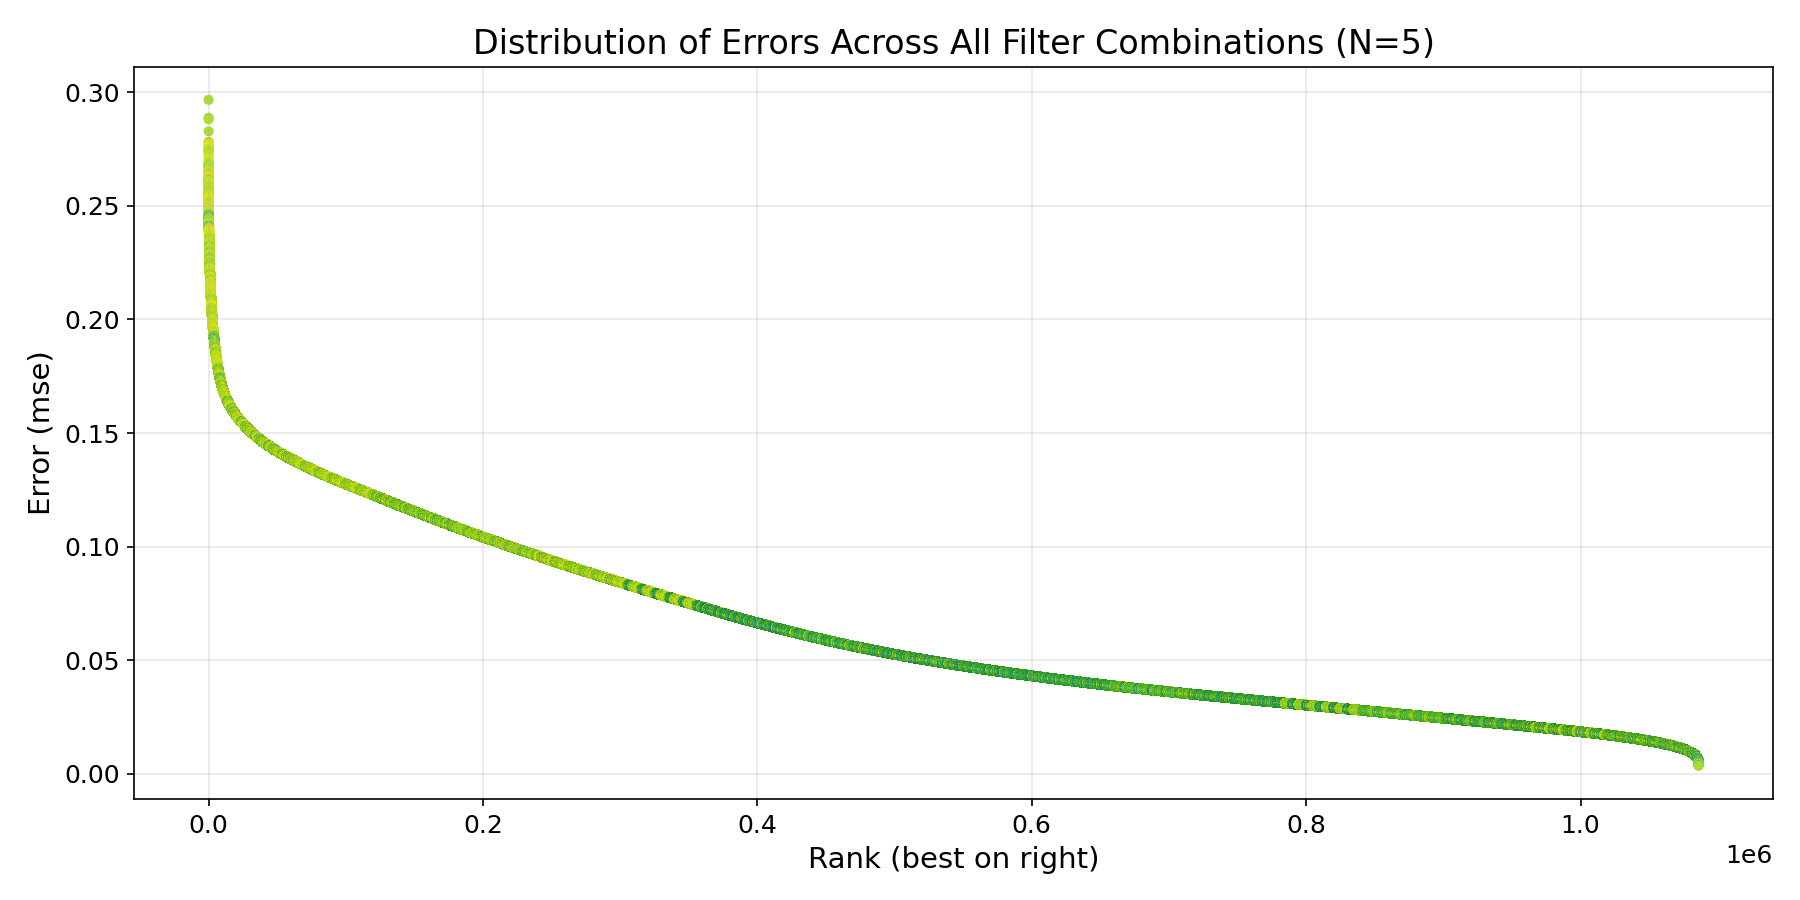
\includegraphics[width=1.05\linewidth]{media/all_errors.png}
    \captionof{figure}{MSE Error distribution across all filter combinations for {\color{red} M}=5}
\end{center}

%not super relevant:
%As the search space grows combinatorially with $N$, we cannot feasibly consider all combinations for large $N$.
%To alleviate this issue, we introduce a 'prune' factor which removes filters based on a cosine similarity metric. 

\subsubsection{PCA Analysis}
To find the optimal filter combination
%for each $N$ 
without brute force search, we can use PCA analysis to find the optimal weights $\mathbf{M}$ for all filters, and then select the top $M$ filters with the highest weights.

%% Kyle I am hoping I am not changing the sense of what your are doing. I commented the next out because I couldn't make it square with the text (as I see it)
%This method effectively creates one $\boldsymbol{M}$ and iteratively reduces weights that can be discarded with minimal loss, until reaching $N$ nonzero entries.  


%%% Graham GOT TO HERE

\subsubsection{Blended Methods} 

While brute force methods guarantee minimum possible loss by investigating the entire search space, large $N$ implementations render this technique impossible. 
Crucially, we can decrease the speed of combinatoric explosion by pruning our set of filters, but the problem of which filter to exclude in a pairwise filter pruning decision is not trivial. 

To address this problem, we use a blended method which suggests a solution using PCA or another heuristic method for $N$ filters, and then greedily considers another set of $N_2$ filters from the remaining set. 
This provides a middle ground to the performance-accuracy tradeoff.
We see that a significant MSE shortfall grows with $N$ as $N_2=0$, but nearly disappears at $N_2>0$ for most practical values of $N$.

Further, certain PCA solutions achieve effectively identical $\Delta E_{2000}$ to those achieved by exhaustive search, especially at $N>4$ and $N_2 \in \{1,2\}$.

\begin{center}
    \centering
    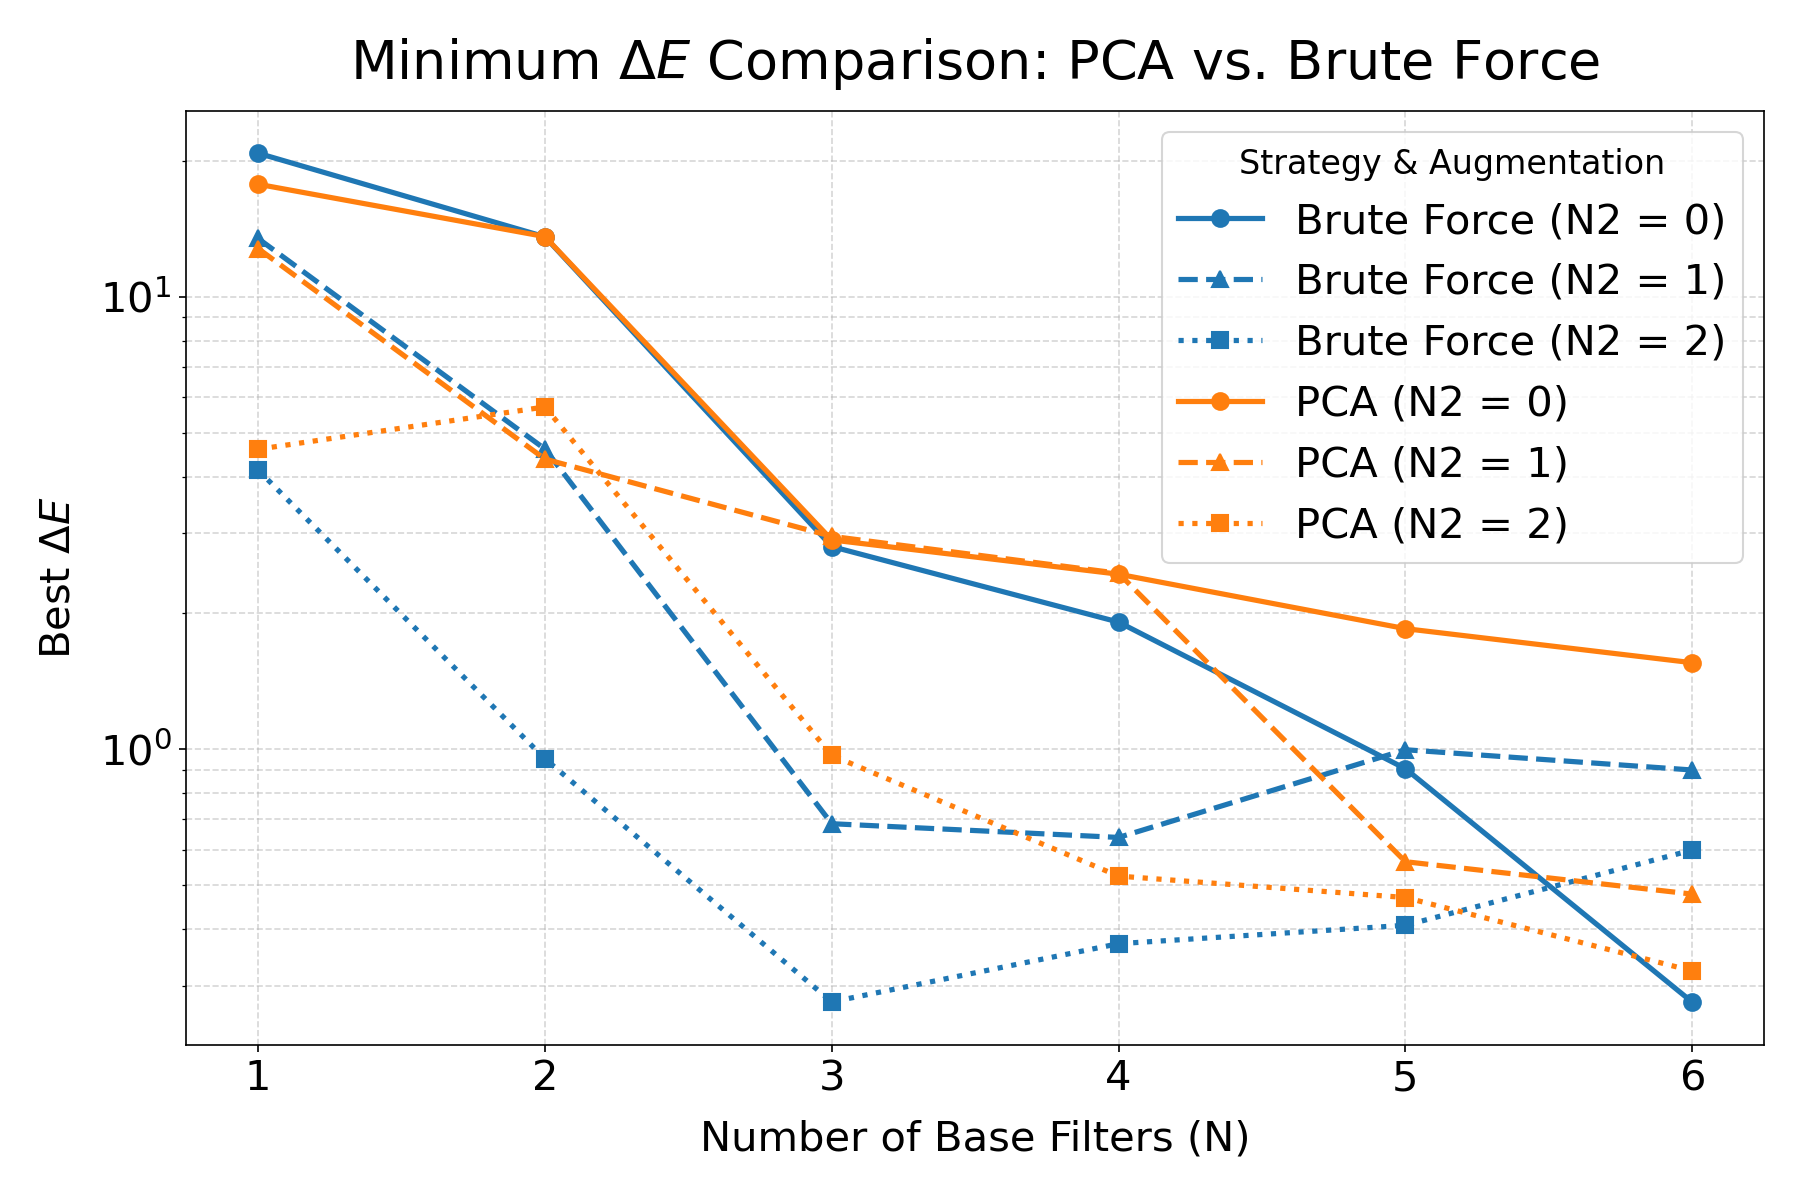
\includegraphics[width=\linewidth]{media/deltaE_comparison_exact_paths.png}
    \captionof{figure}{Comparable $\Delta E_{2000}$ performance between PCA and Exhaustive Search}
\end{center}

We also compare the time performance of these, and demonstrate the significant improvement afforded by PCA, as well as the relative speed of adding 2 layers of brute force searching.
\begin{center}
    \centering
    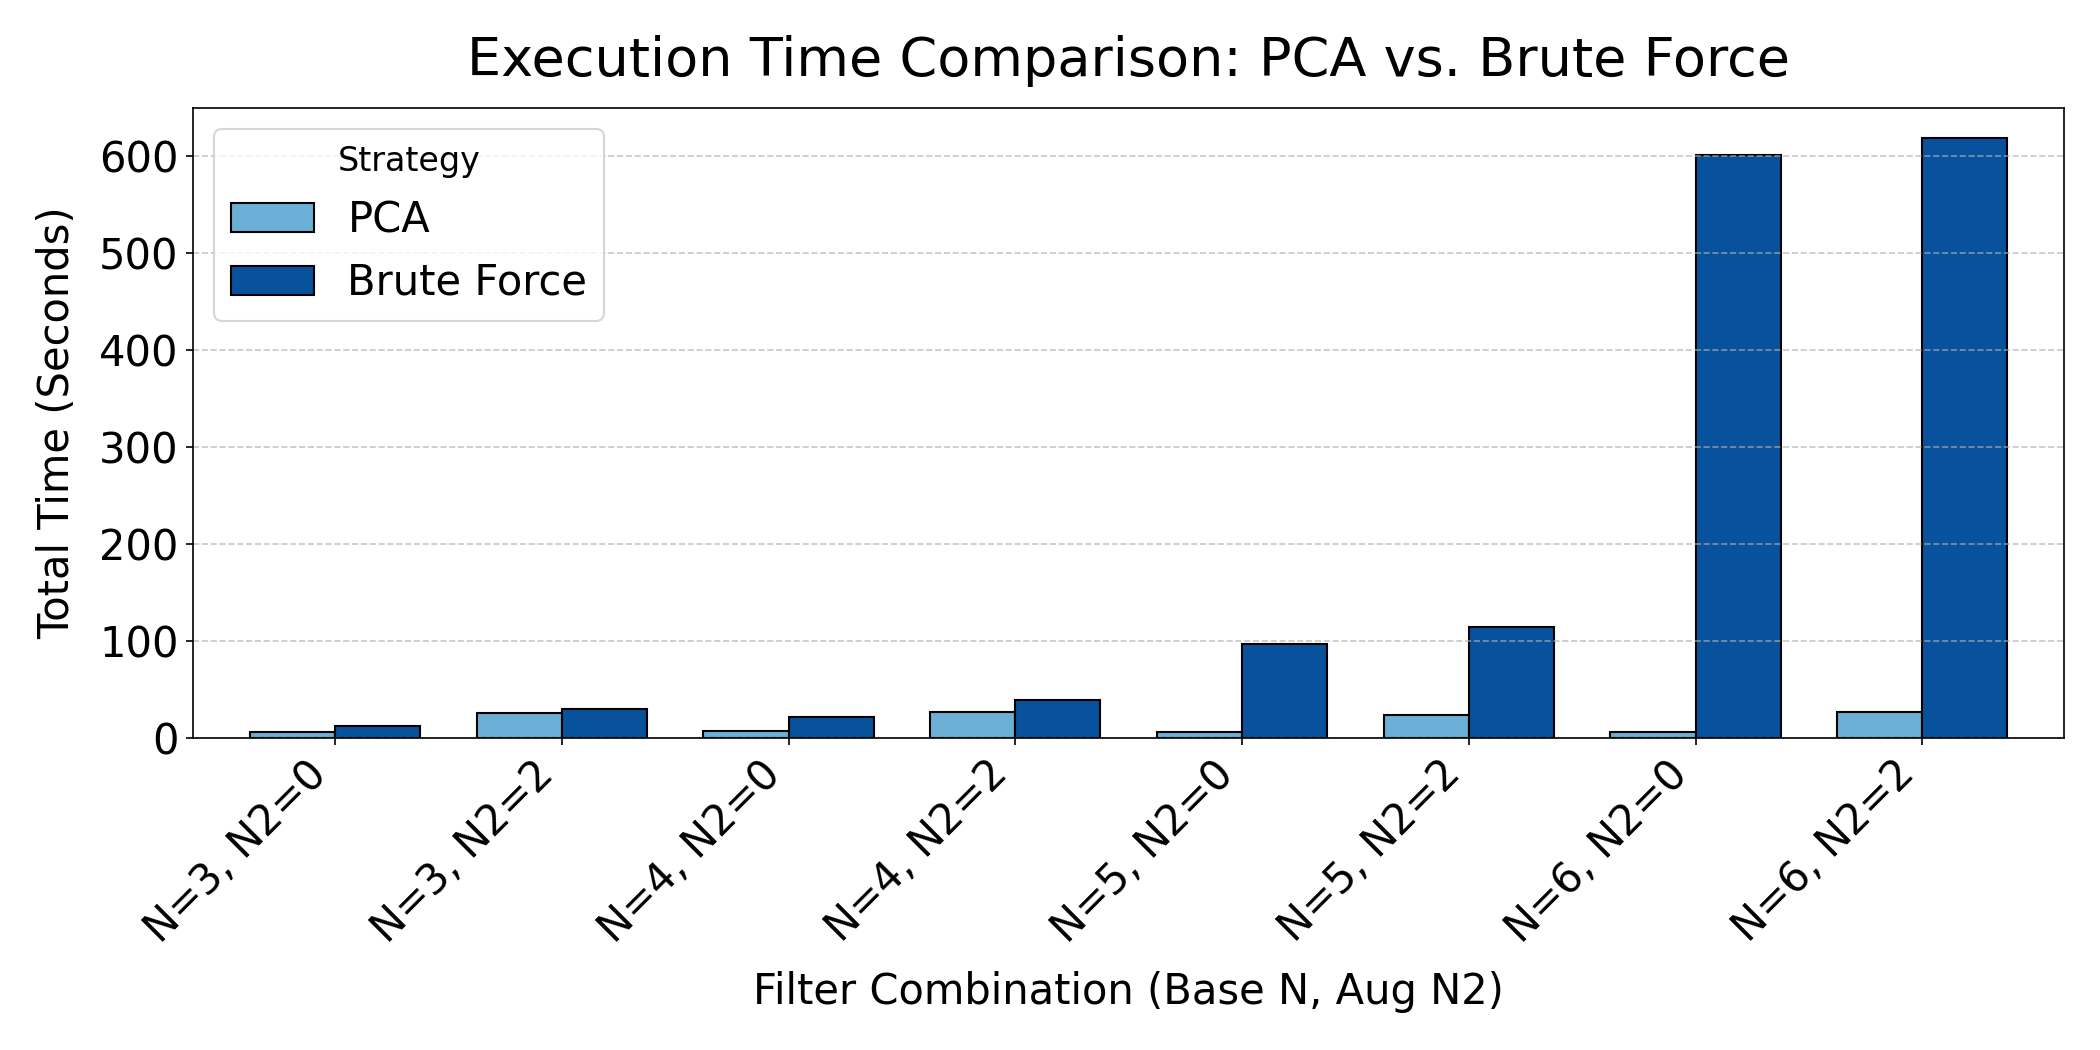
\includegraphics[width=\linewidth]{media/timing_comparison.png}
    \captionof{figure}{Timing Comparison between PCA and Brute Force Selection Methods}
\end{center}
